\chapter{Supplemental Figures and Tables}

\begin{figure}[!ht]
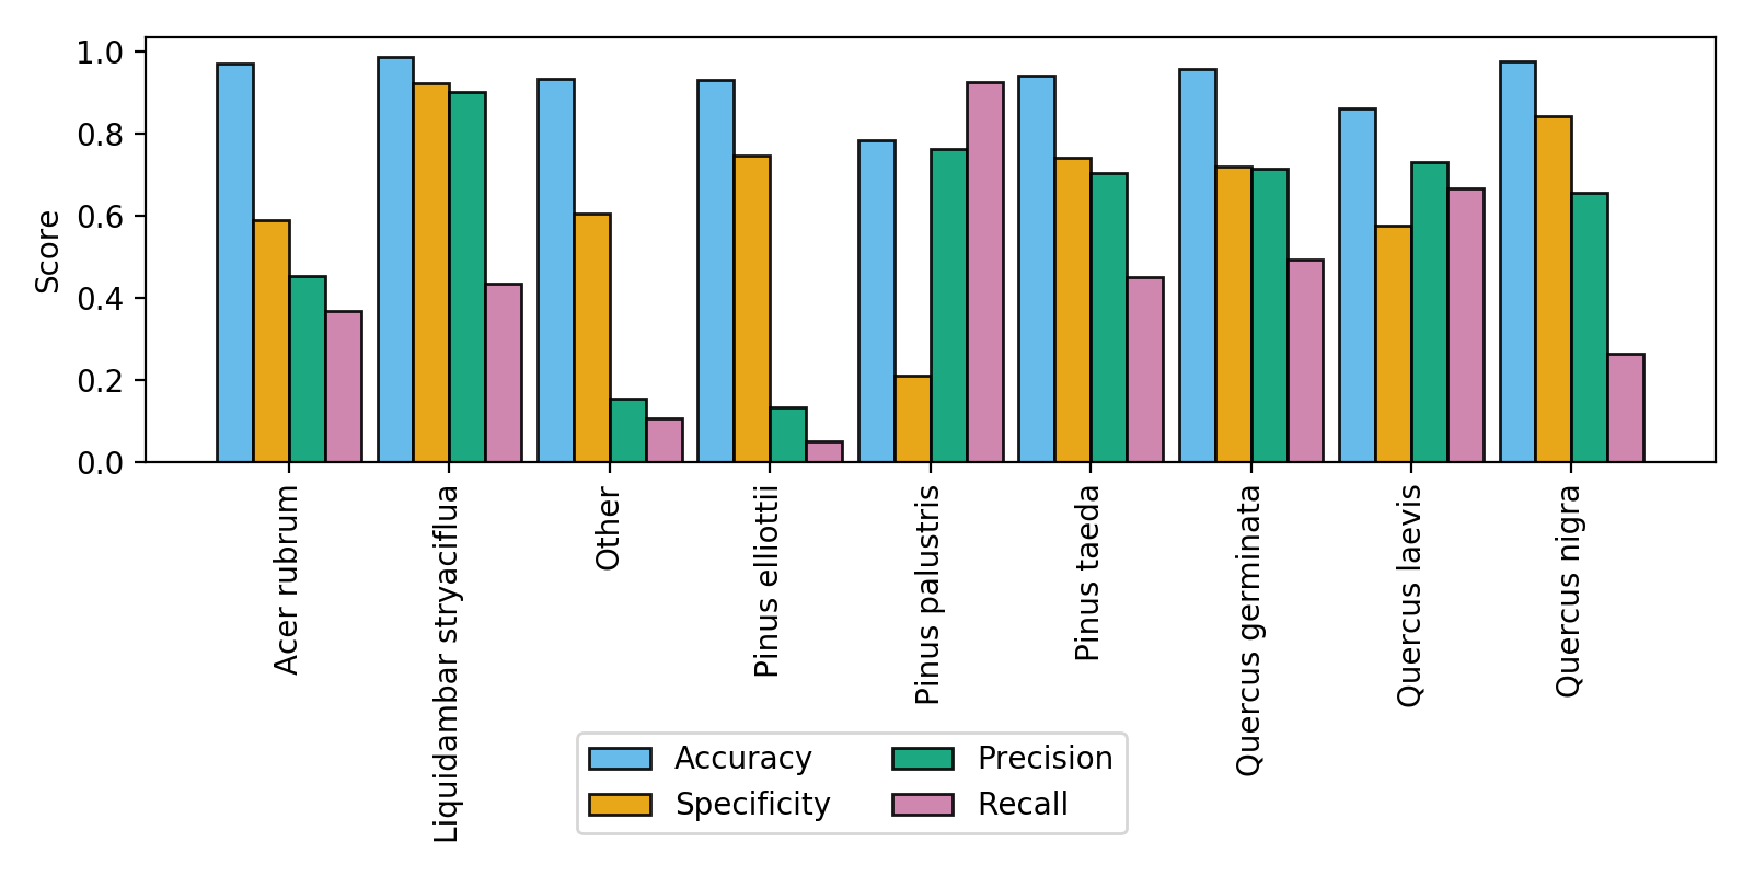
\includegraphics[width=\textwidth]{figures/ch2-performance-continuous.pdf}
\centering
\caption[Per-species secondary model performance metrics applied to test data calculated using per-crown prediction probabilities.]{Per-species secondary model performance metrics applied to test data calculated using per-crown prediction probabilities. Metrics weighted by the true negative rate (i.e., accuracy and specificity) were high for all species since the models correctly predicted the most common species. However, metrics weighted by the true positive rate (i.e., precision and recall) were more variable since there were fewer than six observed crowns for seven of the nine species. This penalized rare species misclassifications.}
\label{fig:performance-continuous}
\end{figure}

\clearpage

\begin{figure}[!ht]
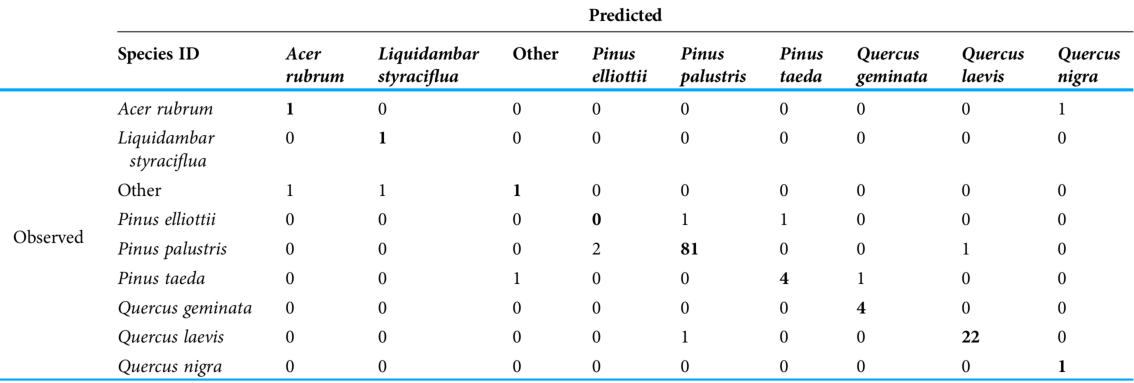
\includegraphics[width=\textwidth]{figures/ch2-confusion-matrix.pdf}
\centering
\caption[Confusion matrix computed from the binary classification results of the CCB-ID model on the competition test data.]{Confusion matrix computed from the binary classification results of the CCB-ID model on the competition test data. These metrics were calculated using the independent crown data.
Bold entries highlight correct model predictions.}
\label{fig:confusion-matrix}
\end{figure}

\clearpage

\begin{table}[!ht]
\centering
\footnotesize
\csvautotabular{tables/table-S1.csv}
\caption{List of Satellite Earth observation sensors used to measure biodiversity patterns using the Essential Biodiversity Variables (EBV) framework.}
\label{tab:eo-sensors}
\end{table}

\clearpage

\begin{table}[!ht]
\centering
\csvautotabular{tables/table-S2.csv}
\caption[Sensitivity analysis showing permutation importance scores for 11 environmental features predicting \textit{Aedes} niche preferences.]{Sensitivity analysis showing permutation importance scores for 11 environmental features. Temperature variance is a strong independent predictor of \textit{Aedes albopictus} spatial distributions, and \textit{Ae. aegypti} was less sensitive to permutation in any one variable.  These scores were generated by randomly permuting covariate values one by one, computing loss in model test performance, then scaling and ranking features based on the total range of model performance loss by vector.}
\label{tab:sensitivity-analysis}
\end{table}

\clearpage

\begin{table}[!ht]
\centering
\footnotesize
\csvautotabular{tables/table-S3a.csv}
\caption{Plot locations and abundance records from all \textit{Aedes} and non-\textit{Aedes} mosquito samples.}
\label{tab:plot-locations}
\end{table}

\clearpage

\begin{table}[!ht]
\centering
\footnotesize
\csvautotabular{tables/table-S3b.csv}
\end{table}

\clearpage

\begin{table}[!ht]
%\centering
\footnotesize
\csvautotabular{tables/table-S3c.csv}
\end{table}